% -*- mode: LaTeX; TeX-PDF-mode: t; -*- # Tell emacs the file type (for syntax)
% Add the listed directories to the search path
% (allows easy moving of files around later)
% these paths are searched AFTER local config kpsewhich

% *.sty, *.cls
\makeatletter
\def\input@path{{@resources/texlive/texmf-local/tex/latex/}
        ,{@resources/texlive/texmf-local/bibtex/bst/},
        ,{@resources/texlive/texmf-local/bibtex/bib/},
        ,{@local/}
        }
\makeatother
\makeatletter
\def\bibinput@path{{@resources/texlive/texmf-local/tex/latex/}
        ,{@resources/texlive/texmf-local/bibtex/bst/},
        ,{@resources/texlive/texmf-local/bibtex/bib/},
        ,{@local/}
        }
\makeatother
 % allow latex to find custom stuff
\input{./.econtexRoot}
\documentclass{beamer}
\newcommand{\texname}{SolvingMicroDSOPs-Slides}
\usepackage{local-macros}      % defns for this project
\usepackage{econark}           % econark defns
\usepackage{llorracc-handouts} % allow references to llorracc-handouts
\usepackage{owner}             % llorracc or econ-ark?
\usepackage{local-packages}    % LaTeX config in ./resources/latex
\provideboolean{MPCMatchVersion}\setboolean{MPCMatchVersion}{true}
\newcommand{\MPCMatch}{\ifthenelse{\boolean{MPCMatchVersion}}}

\usepackage[Overlays]{optional}
%\usepackage{\local}
\usepackage{ulem}   % used in slides

\usepackage{econtexShortcuts}
\usepackage{econark}

% if this is uncommented, bullets are shown step by step; comment out to make printable version:
\beamerdefaultoverlayspecification{<+->}

%\usepackage{\texname-options}
% if invoked from shell with option NoOverlays, make printable version
% (no partial slides where bullets unfold)
\opt{NoOverlays}{\setboolean{WithOverlays}{false}\beamerdefaultoverlayspecification{}}

% Jirka's definitions
\definecolor{jirkasred}{rgb}{0.9,0,0}
\newcommand{\jemph}[1]{{\color{jirkasred}#1}}
\def\newblock{\hskip .11em plus .33em minus .07em}

\mode<presentation>
{
  \usetheme{default}
  % or ...
  \setbeamercovered{transparent}
}

%\setbeamertemplate{navigation symbols}{}  % Take away navigation symbols

\usetheme{Frankfurt}

%_____________ Opening slide _______________________

\begin{document}

\title[SolvingMicroDSOPs]{\textbf{Structural Estimation of Dynamic Stochastic\\ Optimizing Models of Intertemporal Choice \\ \LARGE{For Dummies!}}}
\author[Carroll]{Christopher Carroll\inst{1}}

\institute{
  \inst{1} Johns Hopkins University and NBER\\   \texttt{ccarroll@jhu.edu} \and
    }
\date{June 2012 \\ {\tiny \url{http://www.econ2.jhu.edu/people/ccarroll/SolvingMicroDSOPs-Slides.pdf}}
}


\begin{frame}[plain]
  \titlepage
\end{frame}

\section{Introduction}

\begin{frame}
\begin{itemize}
\item Efficient Solution Methods for Canonical $C$ problem
\begin{itemize}
\item CRRA utility
\item Plausible (microeconomically calibrated) uncertainty
\item Life cycle or infinite horizon
\end{itemize}
\item How To Add a Second Choice Variable
\item Method of Simulated Moments Estimation of Parameters
\end{itemize}
\end{frame}

\section{The Problem}

\begin{frame}[label=MaxProb]
\frametitle{\large\textbf{The Basic Problem at Date $t$}}

  \begin{equation}\label{eq:MaxProb}
    \max ~ \Ex_{t}\left[ \sum_{n_{\TranShkEmp}=0}^{T-t} {\DiscAlt}^{n_{\TranShkEmp}} \uFunc({\cLvl}_{t+n})\right],
  \end{equation}

\begin{equation}\begin{gathered}\begin{aligned}
{\yLev}_{\prd}  & = {\pLev}_{\prd}\tranShkEmp_{\prd}
\end{aligned}\end{gathered}\end{equation}
  \begin{equation}\begin{gathered}\begin{aligned}
        \pLvl_{\prdt+1}   = \PermGroFac_{\prdt+1}\pLvl_{\prdt}                                        & \text{~~ -- permanent labor income dynamics} \label{eq:permincgrow}
        \\ \log ~ \tranShkEmp_{\prdt+n}  \sim ~\Nrml(-\std_{\tranShkEmp}^{2}/2,\std_{\tranShkEmp}^{2}) & \text{~~ -- lognormal transitory shocks}~\forall~n>0 .
        %
        \UnifiedNote{Shock space 𝒵ₐᵥ definition; ζₐᵥ = (ψ, θ) with distributions Pₐᵥ}
      \end{aligned}\end{gathered}\end{equation}

\end{frame}

\begin{frame}[label=vrecurse]
\frametitle{\large\textbf{Bellman Equation}}

\begin{eqnarray}
        \vLevBF_{t}(\mLev_{t},\pLev_{t}) & = & \max_{\cLev_{t}}~ \util(\cLev_{t}) + \Ex_{t}[{\DiscAlt} \vLevBF_{t+1}({\mLev}_{t+1},\pLev_{t+1})]\label{eq:vrecurse}
\end{eqnarray}


\begin{equation*}\begin{gathered}\begin{aligned}
   \mLev  & - \text{ `market resources' (net worth plus current income)}
\\ \pLev  & - \text{ permanent labor income }
\end{aligned}\end{gathered}\end{equation*}

\end{frame}

\section{Tricks}
\subsection{Normalization}
\begin{frame}[label=Normalize]
\frametitle{\large\textbf{Trick: Normalize the Problem}}

\begin{eqnarray}
        \null{\vFunc}_{t}({m}_{t}) & = & \max_{{c}_{t}} ~~ \util({c}_{t})+
        \Ex_{t}[{\Discount} \PGro_{t+1}^{1-\CRRA}\null{\vFunc}_{t+1}({m}_{t+1})] \label{vtNorm}
\\         & \text{s.t.} &   \nonumber \\
    {a}_{t}   & = & {m}_{t}-{c}_{t} \nonumber
\\      {m}_{t+1} & = & \underbrace{\left(\Rfree/\PGro_{t+1}\right)}_{\equiv \Rnorm_{t+1}}{a}_{t}+\tShkEmp_{t+1} \nonumber
\end{eqnarray}


where nonbold variables are bold ones normalized by $\pLev$:
\begin{equation}\begin{gathered}\begin{aligned}
\mNrm_{\prd}  & = \mLvl_{\prd}/\pLvl_{\prd}
\end{aligned}\end{gathered}\end{equation}

Yields $\cFunc_{\prd}(m)$ from which we can obtain
\begin{equation}\begin{gathered}\begin{aligned}
  \cLvl_{\prd}(\mLvl_{\prd},\pLvl_{\prd})  & = \cFunc_{\prd}(\mLvl_{\prd}/\pLvl_{\prd})\pLvl_{\prd}
\end{aligned}\end{gathered}\end{equation}

\end{frame}

\begin{frame}[label=Normalize]
\frametitle{\large\textbf{When Doesn't Normalization Work?}}

\begin{itemize}
\item Non-CRRA utility
\item Non-Friedman (transitory/permanent) income process
\begin{itemize}
\item e.g., AR(1)
\item But micro evidence is consistent with Friedman
\end{itemize}
\end{itemize}

\end{frame}
\subsection{View Problem from End of Period}

\begin{frame}[label=Normalize]
\frametitle{Trick: View Everything from End of Period}

Define 
  \begin{equation}\begin{gathered}\begin{aligned}
        \vCntn & = \DiscFac \vArvlNxt(\overbrace{\kNrm_{\prdt+1}}^{\aNrm_{\prdt}}) \label{eq:vEndPrddefn}
\UnifiedNote{tex vCntn = β·𝒜₊(k₊) ≡ ℰ_disc(a); disc stage: ℰ_disc(xₑ) = β·𝒜₊(gₑₐ₊(xₑ)); gₑₐ₊: a → k₊ (pure rename)}
      \end{aligned}\end{gathered}\end{equation}

so 
\begin{equation}\begin{gathered}\begin{aligned}
  \vFunc_{\dcsn(\prd)}(\mNrm_{\prd})  & = \max_{\cNrm_{\prd}}~~ \util(\cNrm_{\prd}) + \vFunc_{\dcsn(\prd)}(\mNrm_{\prd}-\cNrm_{\prd})
\end{aligned}\end{gathered}\end{equation}
with FOC
  \begin{equation}\begin{gathered}\begin{aligned}
        \uFunc^{{c}}({c}_{\stge})   & = \vEndStep^{{a}}({m}_{\stge}-{c}_{\stge}).
        \label{eq:upEqbetaOp}
      \end{aligned}\end{gathered}\end{equation}

and Envelope relation
\begin{eqnarray}
        \util^{\prime}({c}_{t}) & = & \null{\vFunc}^{\prime}_{t}({m}_{t})\label{eq:Envelope}
\end{eqnarray}


\end{frame}


\subsection{Discretization of Risks}
\begin{frame}[label=DiscretizeFig]
\frametitle{Trick: Discretize the Risks}

E.g.\ use an equiprobable 7-point distribution:\medskip\medskip

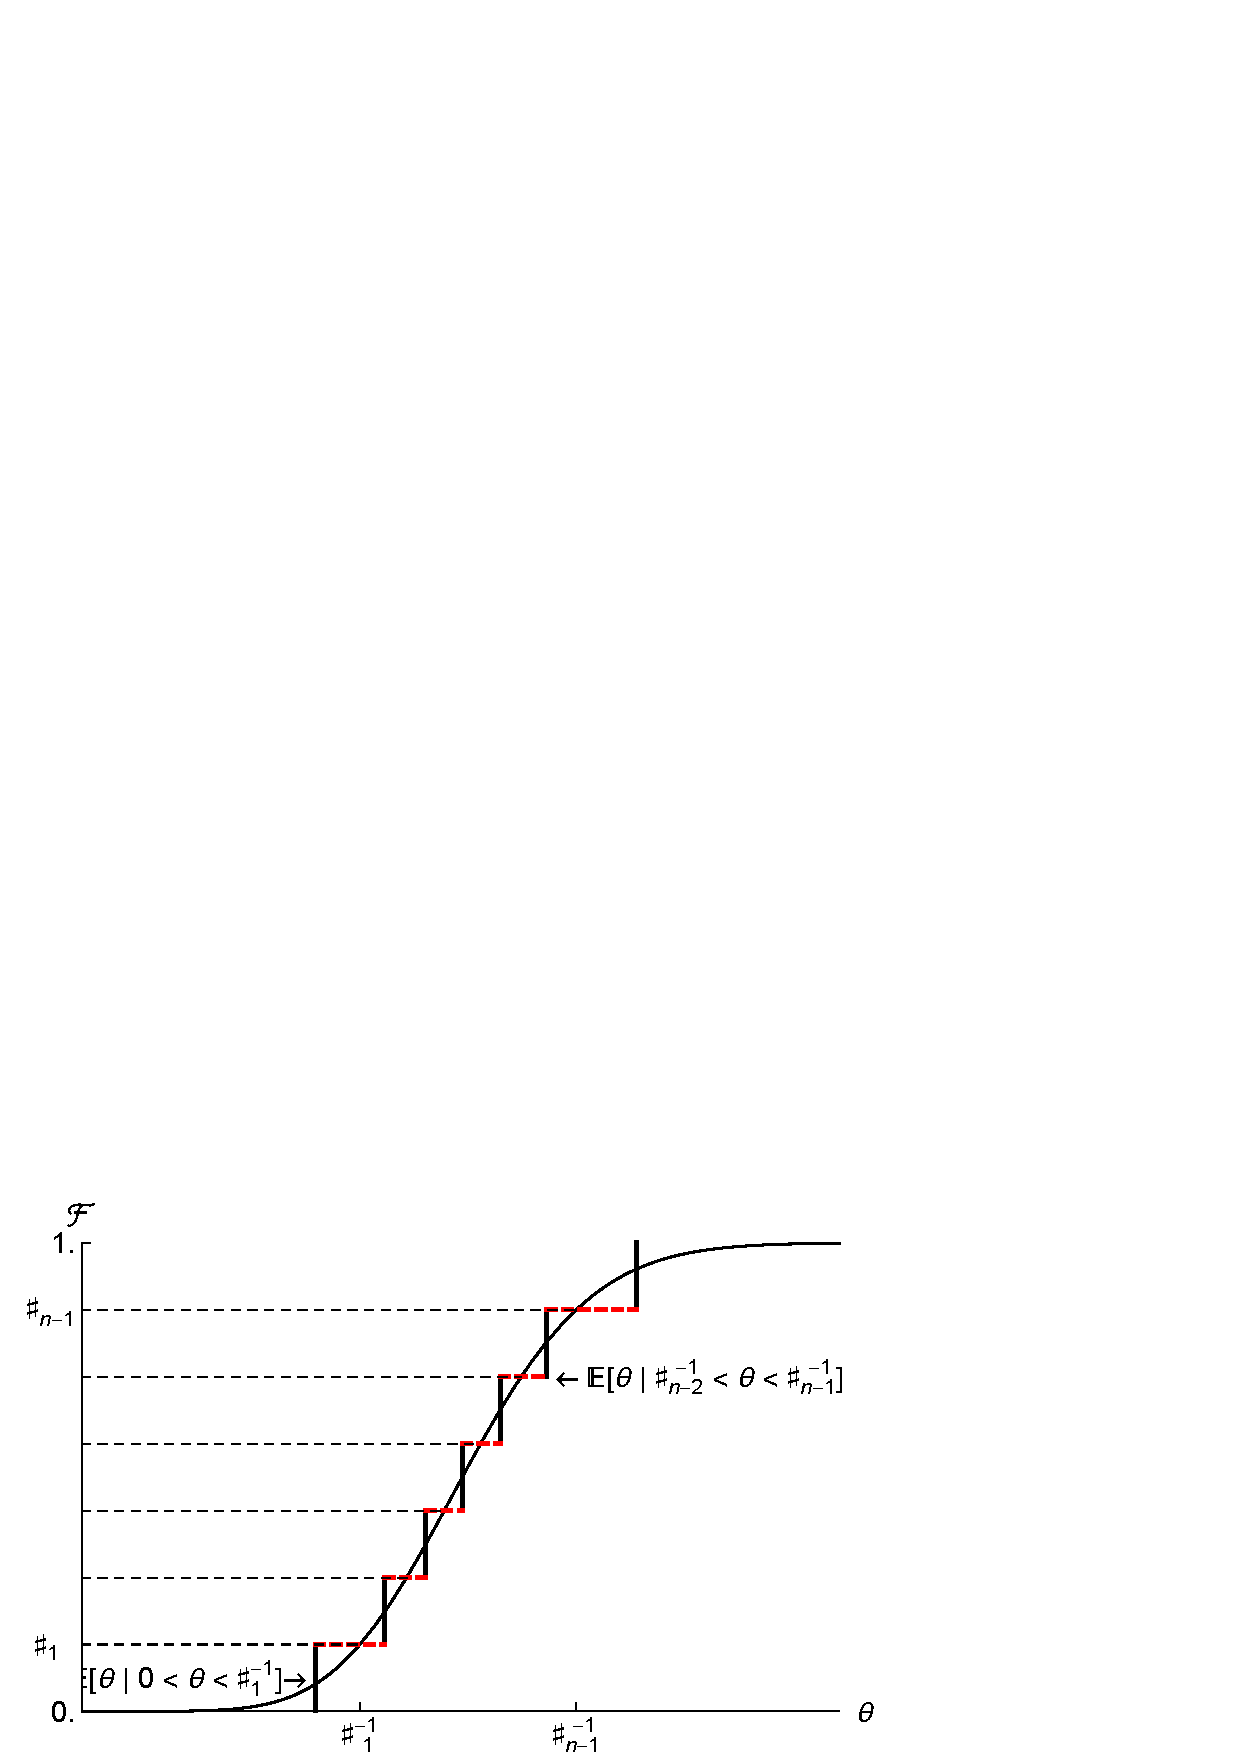
\includegraphics[width=4in]{./Figures/discreteApprox.pdf}

\end{frame}

\begin{frame}[label=DiscretizeEqn]
\frametitle{Trick: Discretize the Risks}

\begin{equation}\begin{gathered}\begin{aligned}
        \vFunc^{\partial}(a_{\prd})  & =  \Discount \Rfree \PermGroFac_{\prd+1}^{-\CRRA} \left(\frac{1}{n}\right) \sum_{i=1}^{n} \util^{\partial}\left(\cFunc_{\prd+1}(\RNrmByG_{\prd+1} a_{\prd} + \tranShkEmp_{i})\right)
\end{aligned}\end{gathered}\end{equation}

%  \begin{equation}\begin{gathered}\begin{aligned}
        \vFunc_{{\cntn}(\prdLst)}(\aNrm)  & =   \DiscFac \PermGroFacAdjV\left(\frac{1}{n_{\tranShkEmp}}\right)\sum_{i=1}^{n_{\tranShkEmp}}   \frac{\left(\RNrmByG_{\prdt} \aNrm + \tranShkEmp_{i}\right)^{1-\CRRA}}{1-\CRRA} \label{eq:vDiscrete}
\UnifiedNote{Numerical approximation of ℰ(xₑ) using discrete Pₐᵥ = {1/n,...,1/n} over 𝒵ₐᵥ = {ζ₁,...,ζₙ}}
      \end{aligned}\end{gathered}\end{equation}


\pause 
So for any particular $\mNrm_{T-1}$ the corresponding $\cNrm_{T-1}$ can be found
using the FOC:
  \begin{equation}\begin{gathered}\begin{aligned}
        \uFunc^{{c}}({c}_{\stge})   & = \vEndStep^{{a}}({m}_{\stge}-{c}_{\stge}).
        \label{eq:upEqbetaOp}
      \end{aligned}\end{gathered}\end{equation}



\end{frame}
\subsection{Interpolate a Consumption Rule}
\begin{frame}
\frametitle{Trick: Interpolate a Consumption Rule}

\begin{enumerate}
\item Define a grid of points $\vctr{\mNrm}$ (indexed $\mNrm[i]$)
\item Use numerical rootfinder to solve 
$\util^{\partial}(\cNrm) = \vFunc^{\partial}_{\prd}(\mNrm[i]-\cNrm)$
\begin{itemize}
\item The $\cNrm$ that solves this becomes $\cNrm[i]$
\end{itemize}
\item Construct interpolating function $\grave{\cFunc}$ by linear interpolation
\begin{itemize}
\item `Connect-the-dots'
\end{itemize}
\end{enumerate}

\end{frame}






\begin{frame}[label=DiscretizeEqn]
\frametitle{Trick: Interpolate a Consumption Rule}

Example: $\vctr{\mNrm}_{T-1} = \{0.,1.,2.,3.,4.\}$ (solid is `correct' soln)

\includegraphics[width=4.0in]{./Figures/PlotcTm1Simple.pdf}

\end{frame}

\begin{frame}[label=vEndPrdSlow]
\frametitle{Problem: Numerical Rootfinding is {\it Slow}}

Numerical search for values of $\cNrm_{T-1}$ satisfying
$\util^{\partial}(\cNrm) = \vFunc^{\partial}_{\prd}(\mNrm[i]-\cNrm)$ at, say,
6 gridpoints of $\vctr{\mNrm}_{T-1}$ may require hundreds or even thousands of
evaluations of
\begin{equation}\begin{gathered}\begin{aligned}
        \vFunc^{\partial}_{T-1}(\overbrace{{m}_{T-1}-\cNrm_{T-1}}^{\aNrm_{T-1}})  & =   \Discount_{T} \PermGroFac_{T}^{1-\CRRA}\left(\frac{1}{n}\right)\sum_{i=1}^{n}   \left( \RNrmByG_{T} a_{T-1} + \tranShkEmp_{i}\right)^{-\CRRA} \notag
\end{aligned}\end{gathered}\end{equation}

\end{frame}




\begin{comment}

\begin{frame}[label=vApprox]
\frametitle{Solution: Approximate \$\vEndPrd\$?}

\pause Given $\{\vctr{\aNrm}_{T-1},\vctr{\EndPrd}_{T-1}\}$, an approximate function $\grave{\EndPrd}_{T-1}$ 
can be constructed by linear interpolation among the points:

\includegraphics[width=4in]{./Figures/PlotOTm1RawVsInt.pdf}

\end{frame}

\begin{frame}
\frametitle{Using $\grave{\EndPrd}_{T-1}$ In Optimization}
\begin{equation*}\begin{gathered}\begin{aligned}
  \vFunc_{\dcsn(\prd)}(\mNrm_{\prd})  & = \max_{\cNrm_{\prd}}~~ \util(\cNrm_{\prd}) + \grave{\EndPrd}_{\prd}(\mNrm_{\prd}-\cNrm_{\prd})
\end{aligned}\end{gathered}\end{equation*}
is {\it much} faster,  but result is bad:
\begin{center}
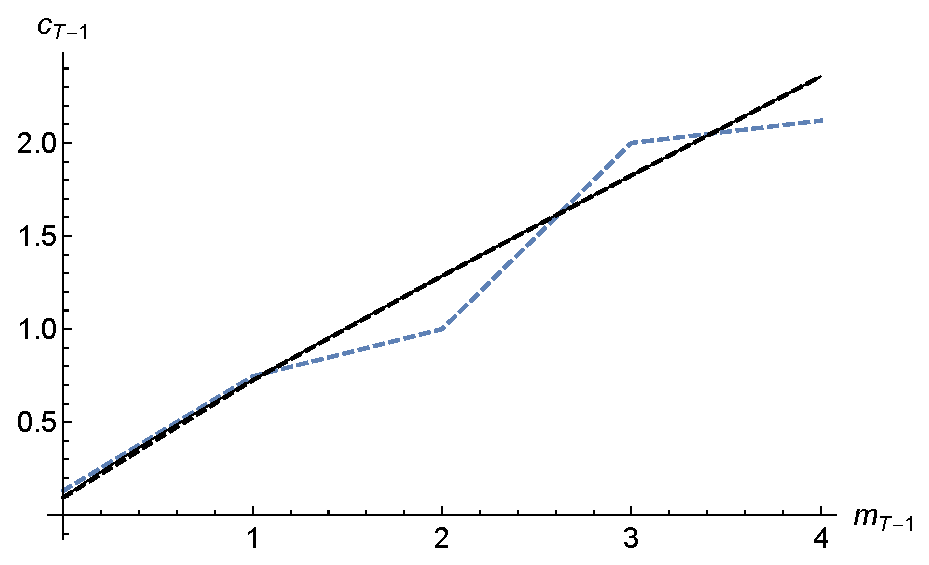
\includegraphics[width=3in]{./Figures/PlotComparecTm1AB}
\end{center}

\end{frame}


\begin{frame}
\frametitle{Approximate $\vFunc^{\partial}(\aNrm)$?}

Better ... but still violates first two principles:
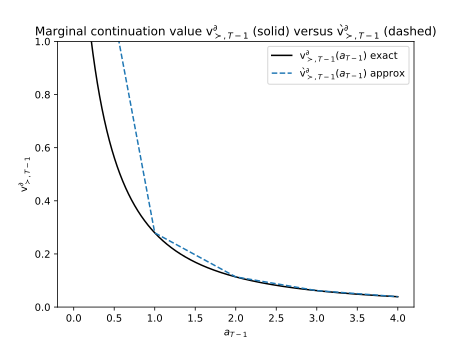
\includegraphics[width=4in]{./Figures/PlotOPRawVSFOC.pdf}

\end{frame}


\end{comment}

\subsection{The Method of Endogenous Gridpoints}
\begin{frame}
\frametitle{Solution: The Method of Endogenous Gridpoints}

\pause 

\begin{itemize}
\item Define vector of {\it end-of-period} asset values $\vctr{\aNrm}$
\item For each $\aNrm[j]$ compute $\vFunc^{\partial}(\aNrm[j])$
\end{itemize}

\pause 

Each of these $\vFunc^{\partial}[j]$ corresponds to a unique
$\cNrm[j]$ via FOC:
\begin{equation}\begin{gathered}\begin{aligned}
  \cNrm[j]^{-\CRRA}  & = \vFunc^{\partial}(\aNrm[j])
\\ \cNrm[j]  & = \left(\vFunc^{\partial}(\aNrm[j])\right)^{-1/\CRRA}
\end{aligned}\end{gathered}\end{equation}

\pause 

But the DBC says
\begin{equation}\begin{gathered}\begin{aligned}
  \aNrm_{\prd}  & = \mNrm_{\prd} - \cNrm_{\prd}
\\ \mNrm[j]  & = \aNrm[j]+\cNrm[j]
\end{aligned}\end{gathered}\end{equation}

\pause 
So computing $\vFunc^{\partial}$ at a vector of $\vctr{\aNrm}$ values has produced for us the corresponding $\vctr{\cNrm}$ and $\vctr{\mNrm}$ 
values at virtually no cost!  

\pause 
\medskip 
From these we can interpolate as before to construct $\grave{\cFunc}_{\prd}(\mRat)$.

\end{frame}


\begin{frame}
\frametitle{Why Directly Approximating $\vFunc_{\dcsn(\prd)}$ is a Bad Idea}

Principles of Approximation

\begin{itemize}
\item Hard to approximate things that approach $\infty$ for relevant $\mNrm$
\begin{itemize}
\item Not a prob for Rep Agent models: `relevant' $\mNrm$'s are $\approx$ SS
\end{itemize}
\item Hard to approximate things that are highly nonlinear 
%\item Best to approximate things that directly govern behavior
\end{itemize}


\end{frame}


\begin{frame}
\frametitle{Approximate Something That Would Be Linear in PF Case}

\medskip

Perfect Foresight Theory:
\begin{equation}\begin{gathered}\begin{aligned}
  \cFunc_{\prd}(\mRat)  & = (\mRat+\hEnd_{\prd})\MPCmin_{\prd} 
\end{aligned}\end{gathered}\end{equation}
for market resources $\mNrm$ and end-of-period human wealth $\hEnd$.


\medskip\medskip
\pause 

This is why it's a good idea to approximate $\cFunc_{\prd}$ 

\pause \medskip\medskip

Bonus: Easy to debug programs by setting $\sigma^{2} = 0$ and
testing whether numerical solution matches analytical!

\end{frame}

\subsection{Approximate Inverted Functions}
\begin{frame}%[ValFnApprox]
\frametitle{But What if You {\it Need} the Value Function?}

Perfect foresight value function:
  \begin{equation}\begin{gathered}\begin{aligned}
        \bar{\vFunc}_{\dcsn(\prdt)}(m_{\prdt})  & = \uFunc(\bar{\cNrm}_{\prdt})\PDVCoverc_{\prdt}^{T}\label{eq:vFuncPF}
        \\  & = \uFunc(\bar{c}_{\prdt}) \MPCmin_{\prdt}^{-1} % 20190820
        \\  & = \uFunc((\aboveMin \mNrm_{\prdt}+\aboveMin \hNrm_{\Cntn})\MPCmin_{\prdt}) \MPCmin_{\prdt}^{-1} % 20190820
        \\  & = \uFunc(\aboveMin \mNrm_{\prdt}+\aboveMin \hNrm_{\Cntn})\MPCmin_{\prdt}^{1-\CRRA} \MPCmin_{\prdt}^{-1} % 20190820
        \\  & = \uFunc(\aboveMin \mNrm_{\prdt}+\aboveMin \hNrm_{\Cntn})\MPCmin_{\prdt}^{-\CRRA}  % 20190820
        %
        \UnifiedNote{𝒱(xᵥ) (partial: upper-bound perfect foresight decision-value function for MoM)}
      \end{aligned}\end{gathered}\end{equation}

  This can be transformed as
  \begin{equation*}\begin{gathered}\begin{aligned}
        \bar{\vInv}_{\prdt}  & \equiv  \left((1-\CRRA)\bar{\vFunc}_{\dcsn(\prdt)}\right)^{1/(1-\CRRA)}
        \\  & = \cNrm_{\prdt}(\PDVCoverc_{\prdt}^{T})^{1/(1-\CRRA)}
        \\  & = (\aboveMin \mNrm_{\prdt}+\aboveMin \hNrm_{\Cntn})\MPCmin_{\prdt}^{-\CRRA/(1-\CRRA)}   % 20190820
      \end{aligned}\end{gathered}\end{equation*}

which is linear.  

\medskip\medskip
\pause If you need the value function, approximate the {\it inverted} value function to generate $\grave{\vInv}_{\prd}$ 
and then obtain your approximation from 
\begin{equation}\begin{gathered}\begin{aligned}
  \grave{\vFunc}_{\dcsn(\prd)}  & = \util(\grave{\vInv}_{\prd})
\end{aligned}\end{gathered}\end{equation}


\end{frame}

\subsection{Derivatives}
\begin{frame}
\frametitle{Approximate Slope Too}

\cite{BufferStockTheory} shows that $\cFunc^{\dm}_{\prd}$ exists everywhere.
\medskip

\pause 
Define {\it consumed} function and its derivative as 
\begin{equation}\begin{gathered}\begin{aligned}
  \cEndFunc_{\prd}(\aNrm)  & = (\vFunc^{\partial}_{\prd}(\aNrm))^{-1/\CRRA}
\\ \cEndFunc_{\prd}^{\partial}(\aNrm)  & = -(1/\CRRA)\left(\vFunc^{\partial}(a)\right)^{-1-1/\CRRA} \vFunc^{\partial\partial}(\aNrm) 
\end{aligned}\end{gathered}\end{equation}

\pause 
and using chain rule it is easy to show that
\begin{equation}\begin{gathered}\begin{aligned}
 \cFunc^{\dm}_{\prd}  & = \cEndFunc^{\partial}_{\prd}/(1+\cEndFunc^{\partial}_{\prd})
\end{aligned}\end{gathered}\end{equation}

\end{frame}

\begin{frame}
\frametitle{To Implement: Modify Prior Procedures in Two Ways}
\begin{enumerate}
\item Construct $\vctr{\cFunc}^{\mNrm}_{\prd}$ along with $\vctr{\cFunc}_{\prd}$ in EGM algorithm
\item Approximate $\cFunc_{\prd}(m)$ using piecewise Hermite polynomial
\begin{itemize}
\item Exact match to both level and derivative at set of points
\end{itemize}
\end{enumerate}
\end{frame}


\subsection{Improving the $\aNrm$ Grid}

\begin{frame}
\frametitle{Problem: $\Alt{\cFunc}$ Below Bottom $\mNrm$ Gridpoint and Extrapolation}

Consider what happens as $a_{T-1}$ approaches $\Min{a}_{T-1}\equiv-\Min{\tranShkEmp}\RNrmByG_{T}^{-1}$,
\begin{equation*}\begin{gathered}\begin{aligned}
        \lim_{{\aNrm} \downarrow \Min{a}_{T-1}} \vFunc{T-1}^{\partial}(\aNrm) 
& =         \lim_{{\aNrm} \downarrow \Min{a}_{T-1}} \Discount \Rfree \PermGroFac_{T}^{-\CRRA} \left(\frac{1}{n}\right) \sum_{i=1}^{n} \left(  \aNrm\RNrmByG_{T}+ \tranShkEmp_{i}\right)^{-\CRRA}
\\  & = \infty
\end{aligned}\end{gathered}\end{equation*}

This means our lowest value in $\vctr{\aNrm}_{T-1}$ should be $> \Min{\aNrm}_{T-1}$.  

\medskip
Suppose we construct $\Alt{\cFunc}$ by linear interpolation:
\begin{equation*}\begin{gathered}\begin{aligned}
  \Alt{\cFunc}_{T-1}(\mRat)  & = \Alt{\cFunc}_{T-1}(\vctr{\mNrm}_{T-1}[1])+\Alt{\cFunc}_{T-1}^{\partial}(\vctr{\mNrm}_{T-1}[1])(\mNrm-\vctr{\mNrm}_{T-1}[1]) \label{eq:ExtrapLin}
\end{aligned}\end{gathered}\end{equation*}

True $\cFunc$ is strictly concave 
$\Rightarrow \exists \mRat^{-} > \Min{\mNrm}_{T-1}$  for which $\mRat^{-}-\Alt{\cFunc}_{T-1}(\mRat^{-}) < \Min{\aNrm}_{T-1}$

\end{frame}

\begin{frame}
\frametitle{Solution: Hard-Code the Bottom Point}

Theory says that
\begin{equation}\begin{gathered}\begin{aligned}
  \lim_{\mRat \downarrow \Min{\mNrm}_{T-1}} \cFunc_{T-1}(\mRat)  & = 0
\\ \lim_{\mRat \downarrow \Min{\mNrm}_{T-1}} \cFunc_{T-1}^{\mNrm}(\mRat)  & = \MPCmax_{T-1}
\end{aligned}\end{gathered}\end{equation}

\medskip 

\begin{enumerate}
\item Redefine $\vctr{\aNrm}$ {\it relative} to $\Min{\aNrm}_{T-1}$
\item Construct corresponding $\vctr{\mNrm}_{T-1}$ and $\vctr{\cNrm}_{T-1}$
\item Prepend $\Min{\mNrm}_{T-1}$ to $\vctr{\mNrm}_{T-1}$
\item Prepend $0.$ to $\vctr{\cNrm}_{T-1}$
\item Prepend $\MPCmax_{T-1}$ to $\vctr{\MPC}_{T-1}$
\end{enumerate}
then proceed as before.

\end{frame}

\begin{frame}
\frametitle{Trick: Improving the $\aNrm$ Grid}
Grid Spacing: Uniform

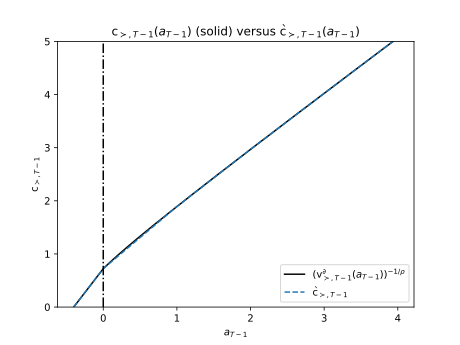
\includegraphics[width=4in]{./Figures/GothVInvVSGothC.pdf}

\end{frame}


\begin{frame}
\frametitle{Trick: Improving the $\aNrm$ Grid}
Grid Spacing: Same $\{\Min{\aNrm},\bar{\aNrm}\}$ But Triple Exponential $e^{e^{e^{...}}}$ Growth

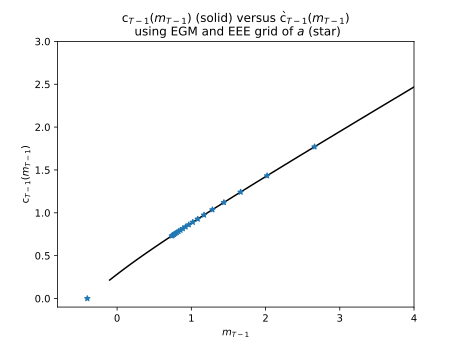
\includegraphics[width=4in]{./Figures/GothVInvVSGothCEEE.pdf}

\end{frame}


\subsection{The Method of Moderation}

\begin{frame}[label=MoM]
\frametitle{The Method of Moderation}

\begin{itemize}
\item Further improves speed and accuracy of solution
\item See my talk at the conference!
\end{itemize}

\end{frame}

\begin{frame}
\frametitle{Imposing `Artificial' Borrowing Constraints}
\begin{equation*}\begin{gathered}\begin{aligned}
{\vFunc}_{T-1}(m_{T-1})  & = \max_{\cNrm_{T-1}} ~~ \util(c_{T-1}) + \Ex_{T-1} [\Discount \PermGroFac_{T}^{1-\CRRA}\vFunc_{T}(m_{T})] \label{eq:ConstrArt}
\\ & \mbox{s.t.}  \nonumber
\\ a_{T-1}  & = m_{T-1} - c_{T-1}
\\ m_{T}  & = \RNrm_{T} a_{T-1} + \TranShkEmp_{T}
\\ a_{T-1} & \geq  0 .
\end{aligned}\end{gathered}\end{equation*}


\pause 

Define $\grave{\cFunc}^{*}_{\prd}$ as soln to unconstrained problem.  Then
  \begin{equation}\begin{gathered}\begin{aligned}
    \grave{\cFunc}_{T-1}({m}_{T-1})  & = \min[{m}_{T-1},\grave{\cFunc}^{\ast}_{T-1}({m}_{T-1})] \label{eq:LiqCons}.
  \end{aligned}\end{gathered}\end{equation}


\end{frame}

\begin{frame}
\frametitle{Imposing `Artificial' Borrowing Constraints}

Point where constraint makes transition from binding to not is
\begin{equation*}\begin{gathered}\begin{aligned}
    \util^{\partial}(\mNrm_{T-1}^{\#})  & = \vFunc^{\partial}_{T-1}(0.)
\\  \mNrm_{T-1}^{\#}  & = \left(\vFunc^{\partial}_{T-1}(0.)\right)^{-1/\CRRA}
\end{aligned}\end{gathered}\end{equation*}
\pause\medskip

Procedure is very easy:
\begin{itemize}
\item Add $0.$ as first point in $\vctr{\aNrm}$
\item $\Rightarrow \vctr{\mNrm}[1] = \mNrm_{T-1}^{\#}$
\item Above $\mNrm_{T-1}^{\#}$, $\grave{\cFunc}_{T-1}(\mRat)$ obtained as before
\item Below $\mNrm_{T-1}^{\#}$, $\grave{\cFunc}_{T-1}(\mRat)=\mNrm$
\end{itemize}

\end{frame}

\begin{frame}
\frametitle{Imposing `Artificial' Borrowing Constraints}
\begin{figure}
\includegraphics[width=4in]{./Figures/cVScCon.pdf}
        \caption{Constrained (solid) and Unconstrained (dashed) Consumption}
        \label{fig:cVScCon}
\end{figure}

\end{frame}

\begin{frame}%[Recursion]
\frametitle{Recursion: Period $t$ Solution Given Period $t+1$}
\begin{enumerate}
\item Construct 
\begin{eqnarray}
        \cEndFunc_{t,i} & = & \left(\vEnd_{t}^{\prime}({a}_{t,i})\right)^{-1/\CRRA},
\\                            & = & \left(\Discount \Ex_{t} \left[\Rfree \PGro_{t+1}^{-\CRRA}(\grave{\cFunc}_{t+1}(\Rnorm_{t+1} {a}_{t,i} +      {\tShkEmp}_{t+1}))^{-\CRRA}\right]\right)^{-1/\CRRA}, \label{eq:vEndeq}
\MPCMatch{\\        \cEndFunc^{a}_{t,i} & = & -(1/\CRRA)\left(\vEnd_{t}^{\prime}({a}_{t,i})\right)^{-1-1/\CRRA} \vEnd_{t}^{\prime\prime}(\aRat_{t,i}),}{}
\end{eqnarray}

\item Call the result $\vctr{\cNrm}_{\prd}$ and generate the corresponding $\vctr{\mNrm}_{\prd}=\vctr{\cNrm}_{\prd}+\vctr{\aNrm}_{\prd}$
\item Interpolate to create $\grave{\cNrm}_{\prd}(\mRat)$
\end{enumerate}

\end{frame}

\begin{frame}%[Convergence]
\frametitle{Consumption Rules $\grave{\cFunc}_{T-n}$ Converge}

\begin{figure}
        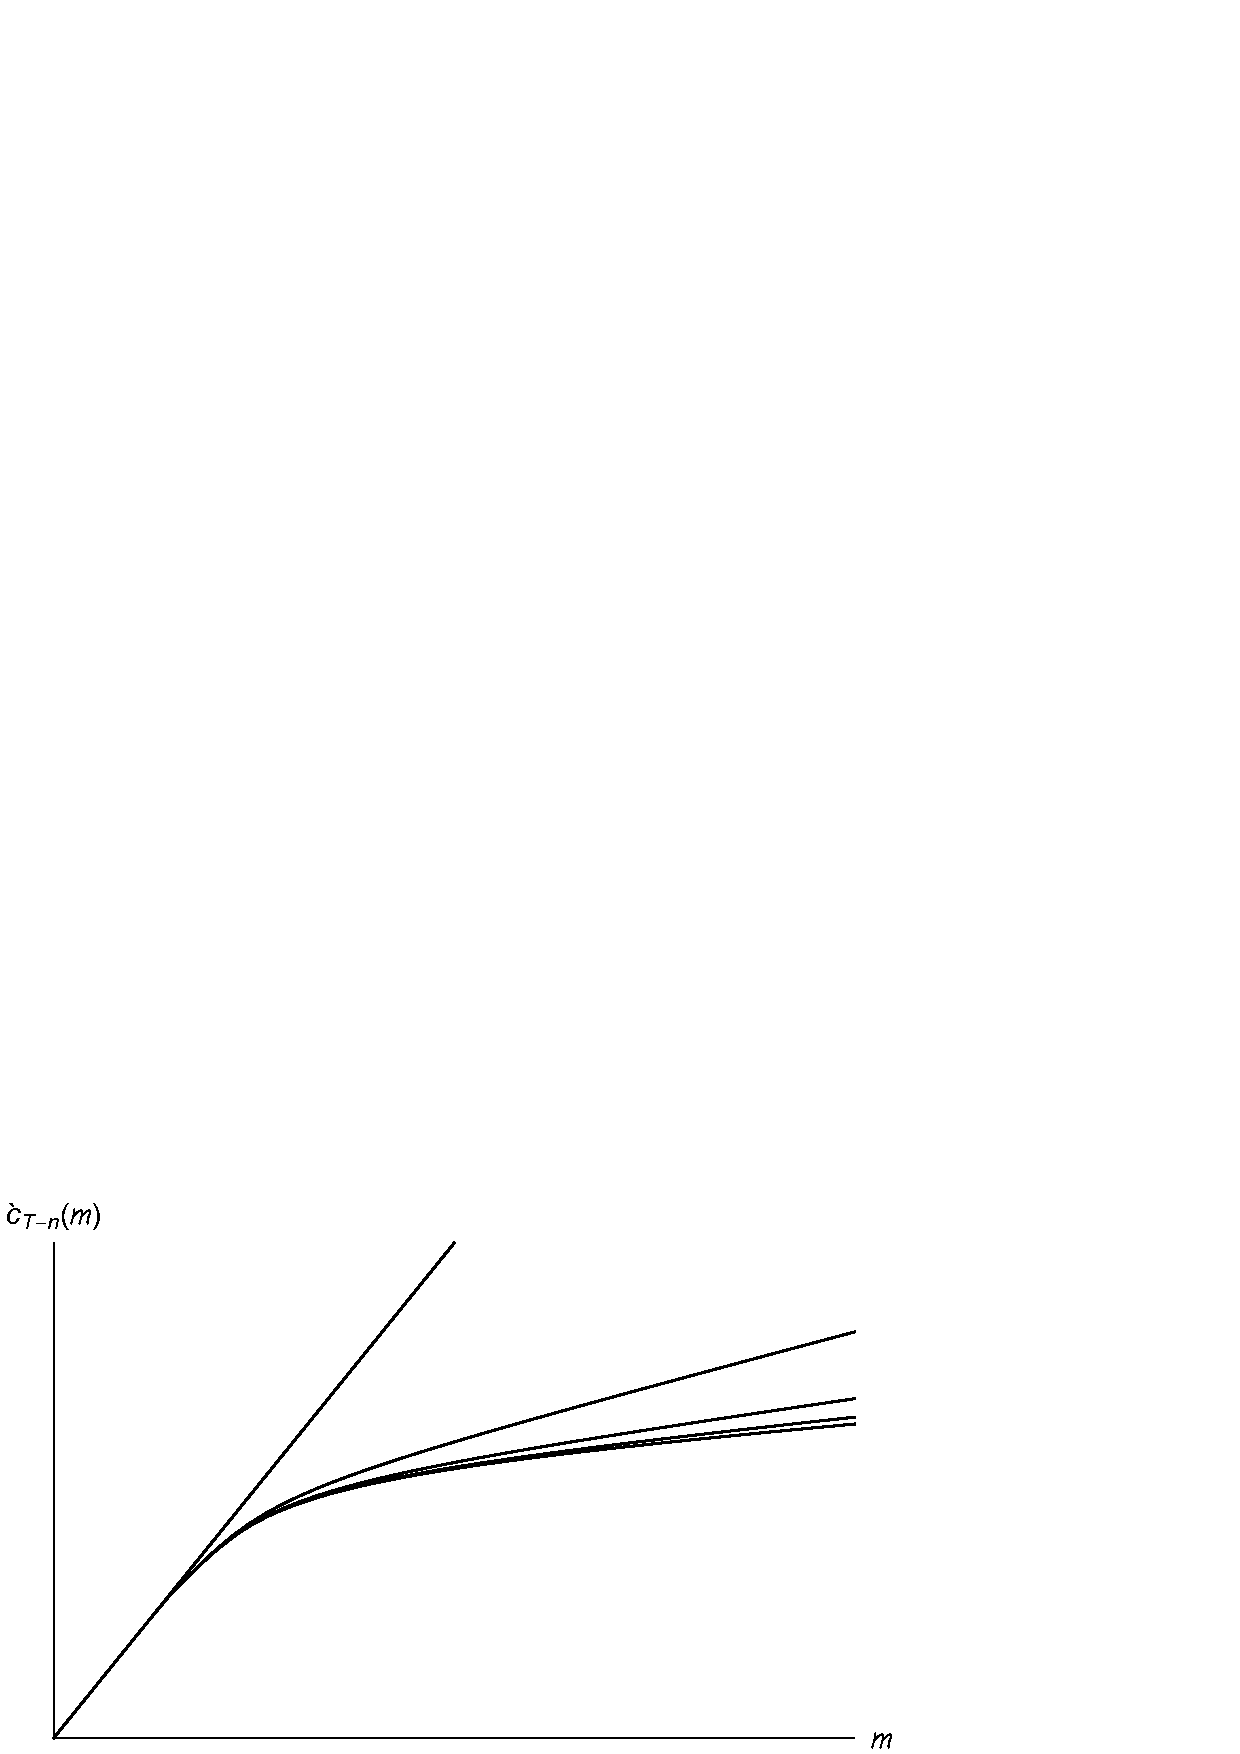
\includegraphics[width=4in]{./Figures/PlotCFuncsConverge.pdf}
        \caption{Converging $\grave{\cFunc}_{T-n}(\mNrm)$ Functions for $n=\{1,5,10,15,20\}$}
        \label{fig:PlotCFuncsConverge}
\end{figure}

\end{frame}


\section{Multiple Control Variables}
\begin{frame}
\frametitle{Portfolio Choice}

Now the consumer has a choice between a risky and a safe asset.  \pause The portfolio
return is
  \begin{equation}\begin{gathered}\begin{aligned}
        \Rport_{t+1}  & = \Rfree(1-\stigma_{t}) + \Risky_{t+1}\stigma_{t} \label{eq:return1}
        \\               & = \Rfree + (\Risky_{t+1}-\Rfree) \stigma_{t} %\label{eq:return2}
      \end{aligned}\end{gathered}\end{equation}

\pause so (setting $\PermGroFac=1$) the maximization problem is \pause 
\begin{eqnarray*}
        {\vFunc}_{t}({m}_{t}) & = & \max_{\{{c}_{t},\varsigma_{t}\}}   ~~ \util({c}_{t}) +  \Discount
        \Ex_{t}[{\vFunc}_{t+1}({m}_{t+1})]
\\      & \text{s.t.} & \nonumber
\\      \Rport_{t+1} & = & \Rfree + (\Risky_{t+1}-\Rfree) \varsigma_{t}
\\      {m}_{t+1} & = & ({m}_{t}-{c}_{t})\Rport_{t+1} + \tShkEmp_{t+1}
\\  0       \leq & \varsigma_{t} & \leq 1, \label{eq:noshorts}
\end{eqnarray*}


\end{frame}

\begin{frame}
\frametitle{Portfolio Choice}

The FOC with respect to $\cNrm_{\prd}$ now yields an Euler equation
  \begin{equation}\begin{gathered}\begin{aligned}
    \util^{\prime}({c}_{t})  & = \Ex_{t}[\Discount {\Rport}_{t+1} \util^{\prime}({c}_{t+1})]. \label{eq:EulercRiskyR}
  \end{aligned}\end{gathered}\end{equation}

\pause
while the FOC with respect to the portfolio share yields
%  \begin{equation}\begin{gathered}\begin{aligned}
    0  & = \Ex_{t}[{\vFunc}_{t+1}^{\prime}({m}_{t+1})(\Risky_{t+1}-\Rfree){a}_{t}] \notag
    \\         & = {a}_{t}\Ex_{t}\left[\util^{\prime}\left(\cFunc_{t+1}({m}_{t+1})\right)(\Risky_{t+1}-\Rfree)\right] \label{eq:FOCw}.
  \end{aligned}\end{gathered}\end{equation}


\end{frame}

\section{The Infinite Horizon}
\subsection{Convergence}
\begin{frame}
\frametitle{Convergence}

When the problem satisfies certain conditions~(\cite{BufferStockTheory}),
it defines a `converged' consumption rule with a `target' ratio $\check{\mNrm}$
that satisfies:
\begin{equation}\begin{gathered}\begin{aligned}
  \Ex_{\prd}[\mNrm_{\prd+1}/\mNrm_{\prd}]  & = 1 \text{~if $\mNrm_{\prd} = \check{\mNrm}$}
\end{aligned}\end{gathered}\end{equation}

\pause 

Define the target $\mNrm$ implied by the consumption rule $\cFunc_{\prd}$ as $\check{\mNrm}_{\prd}$.

\medskip\pause
Then a plausible metric for convergence is to define some value $\epsilon$ and to declare
the solution to have converged when
\begin{equation}\begin{gathered}\begin{aligned}
  |\check{\mNrm}_{\prd+1}-\check{\mNrm}_{\prd}|  & < \epsilon
\end{aligned}\end{gathered}\end{equation}

\end{frame}

\subsection{Tricks}
\begin{frame}
\frametitle{Trick: Coarse then Fine $\tranShkEmp$}

\begin{enumerate}
\item Start with coarse grid for $\tranShkEmp$ (say, 3 points)
\item Solve to convergence; call period of convergence $n$
\item Construct finer grid for $\tranShkEmp$ (say, 7 points)
\item Solve for period $T-n-1$ assuming $\Alt{\cFunc}_{T-n}$ 
\item Continue to convergence
\end{enumerate}

\end{frame}

\begin{frame}
\frametitle{Trick: Coarse then Fine $\vctr{\aNrm}_{T-1}$}

\begin{enumerate}
\item Start with coarse grid for $\vctr{\aNrm}$ (say, 5 gridpoints)
\item Solve to convergence; call period of convergence $n$
\item Construct finer grid for $\vctr{\aNrm}$ (say, 20 points)
\item Solve for period $T-n-1$ assuming $\Alt{\cFunc}_{T-n}$ 
\item Continue to convergence
\end{enumerate}

\end{frame}

\section{Structural Estimation}
\subsection{Life Cycle Model}

\begin{frame}
\frametitle{Life Cycle Maximization Problem}
  \begin{equation*}\begin{gathered}\begin{aligned}
        {\vFunc}_{t}({m}_{t})  & = \max_{{c}_{t}} \left\{\uFunc({c}_{t})+\beth\Alive_{t+1}\hat{\DiscFac}_{t+1}
          \Ex_{t}[(\PermShk_{t+1}\PermGroFac_{t+1})^{1-\CRRA}{\vFunc}_{t+1}({m}_{t+1})] \right\}   \\
        & \text{s.t.} &   \nonumber \\
        {a}_{t}    & = {m}_{t}-{c}_{t} \nonumber
        \\      {m}_{t+1}  & = {a}_{t}\underbrace{\left(\frac{\Rfree}{\PermShk_{t+1}\PermGroFac_{t+1}}\right)}_{\equiv \RNrm_{t+1}}+\TranShkEmp_{t+1}
      \end{aligned}\end{gathered}\end{equation*}

    \begin{equation*}\begin{gathered}\begin{aligned}
      \Alive _{s} &:&\text{probability alive (not dead) until age $s$ given alive at age $s-1$}
      \\      {\hat{\Discount}}_{s} &:&\text{time-varying discount factor between age $s-1$ and $s$}
      \\     \Psi_{s} &:&\text{mean-one shock to permanent income}
      \\     \beth &:&\text{time-invariant discount factor}
    \end{aligned}\end{gathered}\end{equation*}
  

\end{frame}

\begin{frame}
\frametitle{Details follow~\cite{cagettiWprofiles}}
\begin{itemize}
\item Parameterization of Uncertainty
\item Probability of Death
\item Demographic Adjustments to $\Discount$
\end{itemize}
\end{frame}

\begin{frame}
\frametitle{Empirical Wealth Profiles}
\begin{figure}
    \includegraphics[width=3.5in]{./Figures/PlotMeanMedianSCFcollegeGrads.pdf}
    \caption{$\mNrm$ from SCF (means (dashed) and medians (solid))}
    \label{fig:MeanMedianSCF}
\end{figure}
\end{frame}

\begin{frame}
\frametitle{Simulated Moments}

Given a set of parameter values $\{\CRRA,\beth\}$:
\begin{itemize}
\item Start at age 25 with empirical $\mNrm$ data
\item Draw shocks using calibrated $\sigma^{2}_{\permShk}$,$\sigma^{2}_{\tranShkEmp}$
\item Consume according to solved $\cFunc_{\prd}$
\end{itemize}
\pause 
$\Rightarrow \mNrm$ distribution by age
\end{frame}

\begin{frame}
\frametitle{Choose What to Simulate}
    \begin{equation}\begin{gathered}\begin{aligned}
      \lefteqn{    \texttt{GapEmpiricalSimulatedMedians$[\CRRA,\beth]$:=}}      \\
                                                                           &[&\texttt{ConstructcFuncLife$[\CRRA,\beth]$;} \\
                                                                           &\texttt{Simulate;} \\
                                                                           &\sum\limits_{i}^{N}\weight _{i}\left|\varsigma_{i}^{\tau }-\mathbf{s}^{\tau}(\xi )\right|  \\
                                                                           &];&
    \end{aligned}\end{gathered}\end{equation}
  

\end{frame}

\begin{frame}
\frametitle{Calculate Match Between Theory and Data}
\begin{equation}\begin{gathered}\begin{aligned}
\xi  & = \{\CRRA,\beth\}
\end{aligned}\end{gathered}\end{equation}
solve
  \begin{equation}
    \min_{\xi}\sum_{i}^{N}\weight _{i}\left|\wRatio_{i}^{\tau }-\mathbf{s}^{\tau}(\xi )\right|\label{eq:StructEstim}
    %
    \UnifiedNote{[no direct counterpart] (estimation: weighted SMM objective function)}
  \end{equation}


\end{frame}
\begin{frame}
\frametitle{Bootstrap Standard Errors (\cite{horowitzBootstrap})}

Yields estimates of 
\begin{table}[h]
\caption{Estimation Results}\label{tab:EstResults}
\center
\begin{tabular}{cc}
    \hline
    $\CRRA $ & ${\beth}$\\
    \hline
    $4.68$ & $1.00$\\
    $(0.13)$ & $(0.00)$\\
    \hline
\end{tabular}
\end{table}


\end{frame}

\begin{frame}
\frametitle{Contour Plot}
\begin{figure}
     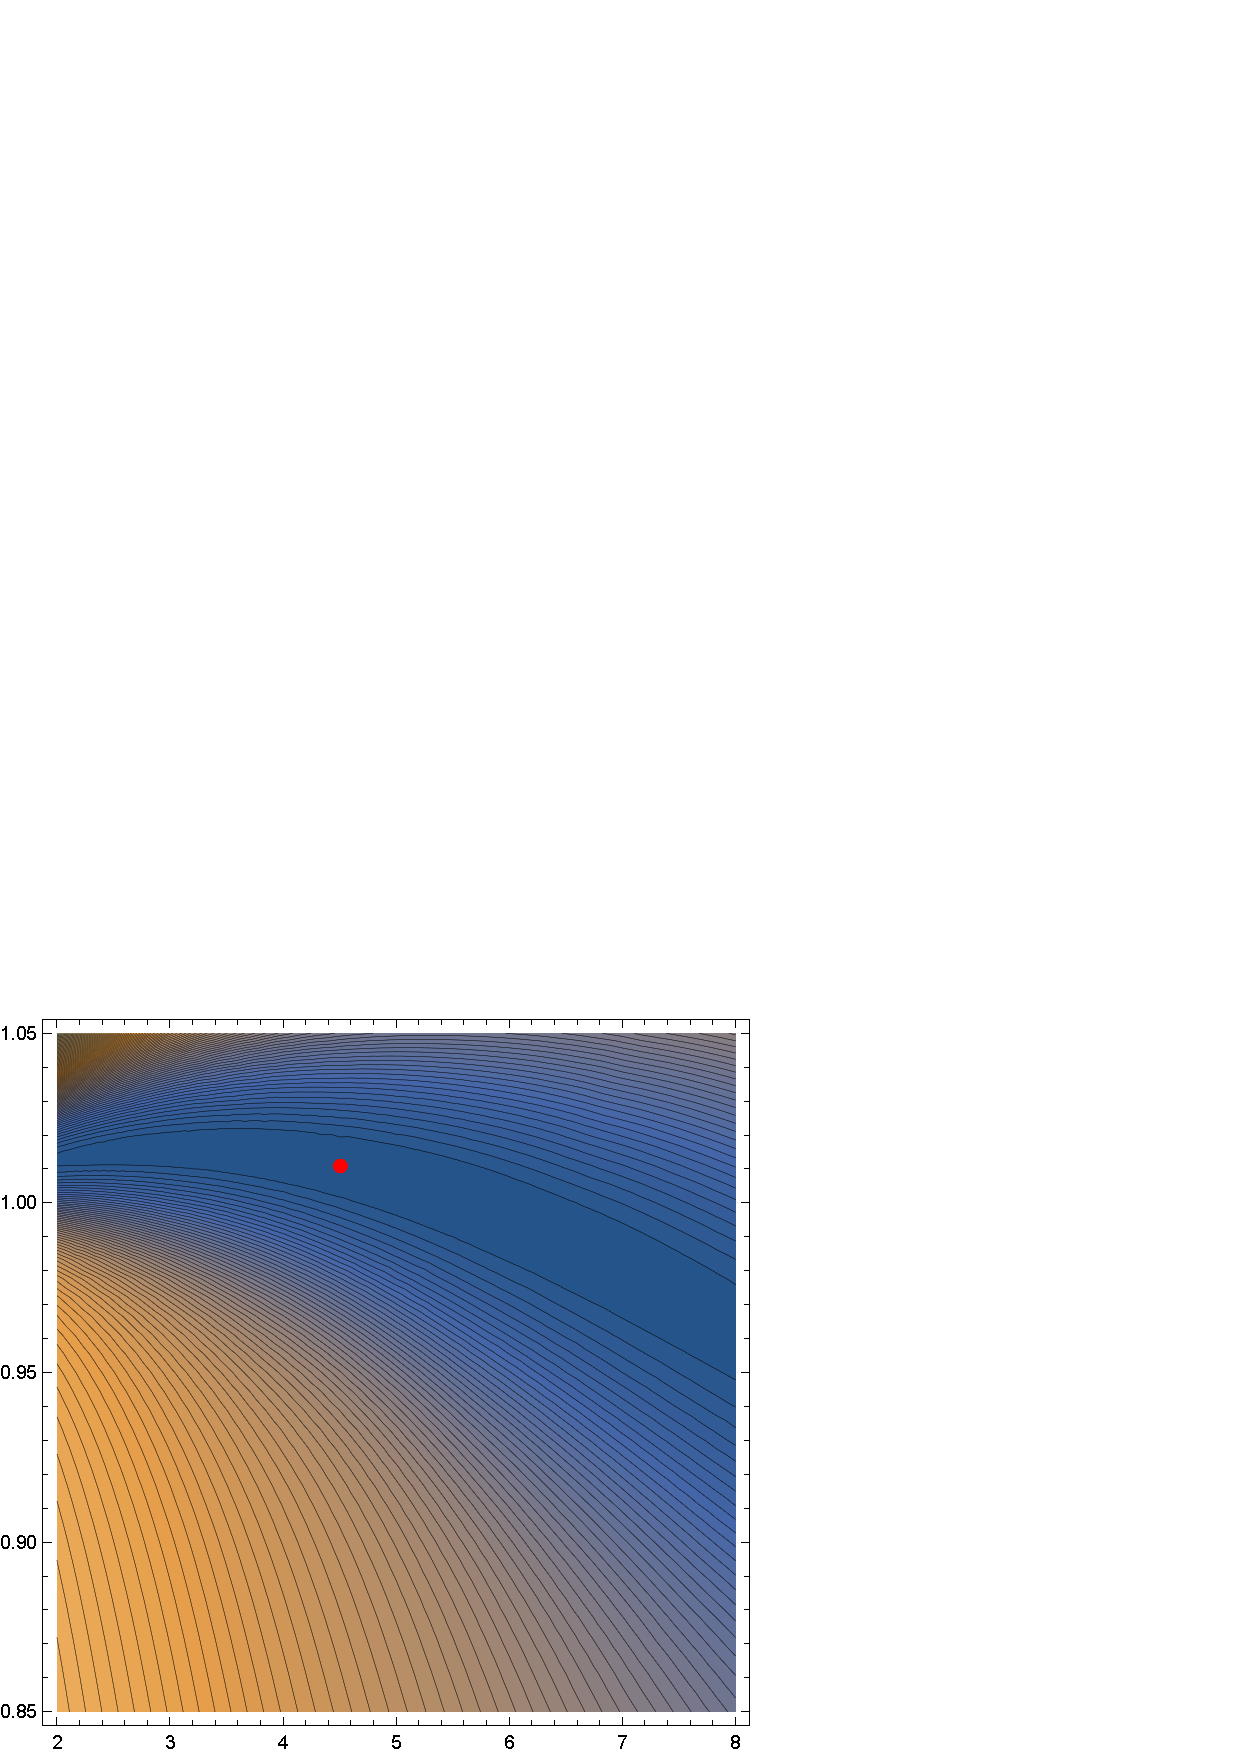
\includegraphics[width=2.5in]{./Figures/PlotContourMedianStrEst.pdf}
    \caption{Point Estimate and Height of Minimized Function}
    \label{fig:PlotContourMedianStrEst}
\end{figure}

\end{frame}

\beamerdefaultoverlayspecification{<*>}

\begin{frame}[allowframebreaks]
\frametitle{\textbf{References}}
\tiny
\input handoutBibMake
\end{frame}


\end{document}
